\documentclass{beamer}

\usepackage[utf8]{inputenc}
\usepackage[magyar]{babel}

\usepackage{lmodern}
\usepackage{amsmath}

\usepackage{wrapfig}

\graphicspath{{images/}}

\usetheme{default}



\setbeamertemplate{navigation symbols}{}

\usecolortheme{whale}

\definecolor{szechenyiblue}{RGB}{35, 76, 171} % define Széchenyi blue

\setbeamercolor*{title}{fg=white}
\setbeamercolor*{author}{fg=white}
\setbeamercolor*{date}{fg=white}
\setbeamercolor*{institute}{fg=white}
\setbeamercolor*{frametitle}{bg=szechenyiblue, fg=white}


\makeatletter
\setbeamertemplate{title page}
{
	\vbox{}
	\begin{centering}

		\begin{beamercolorbox}[sep=8pt,center]{title}
			\usebeamerfont{title}\inserttitle
		\end{beamercolorbox}%
		\begin{beamercolorbox}[sep=8pt,left]{author}
			\usebeamerfont{author}\insertauthor
		\end{beamercolorbox}
		\begin{beamercolorbox}[sep=8pt,left]{institute}
			\usebeamerfont{institute}\insertinstitute
		\end{beamercolorbox}
		\begin{beamercolorbox}[sep=8pt,left]{date}
			\usebeamerfont{date}\insertdate
		\end{beamercolorbox}

	\end{centering}
}
\makeatother

\author{ \underline{Gábor Hanna}, Bérczi Kristóf\inst{1}}
\title{\Huge{Megengedett 2-faktorok sı́kgráfokban}}
\institute[ELTE]
{
	\inst{1}
	ELTE TTK Matematika Intézet,\\
	Operációkutatási tanszék,\\
	Budapest, Magyarország
}
\date{\small{2018. május 29.}}




\begin{document}


{
\usebackgroundtemplate{
\includegraphics[width=1.0\paperwidth]{theme.jpg}}
	\begin{frame}[plain]
		\maketitle
	\end{frame}
}




\begin{frame}{Goddard-Henning sejtés}

	\begin{block}{Sejtés}
		Minden egyszerű, háromszögelt, legalább $4$ csúcsú síkgráfnak létezik olyan $2$-színezése,
		hogy minden csúcsnak mindkét színosztályban van szomszédja.
	\end{block}


	\begin{exampleblock}{Példa}
		Az egyszerűség szükséges.
	\begin{figure}[h]
	  \centering
	  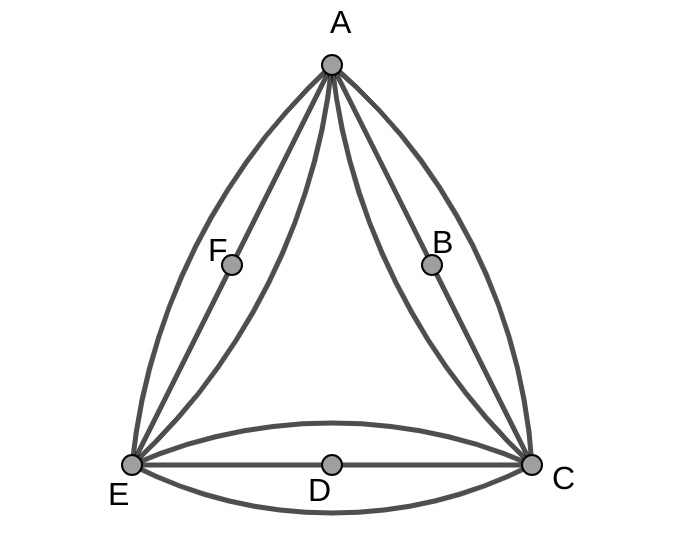
\includegraphics[width=30mm]{parallel}
	\end{figure}
	\end{exampleblock}
\end{frame}

\begin{frame}{Néhány korábbi eredmény}
		\begin{itemize}
			\item Karakterizáció maximális outerplanar gráfokra, ennek segítségével
			a sejtés igazolása Hamilton gráfokra. (Nagy Zoltán Lóránt)
			\begin{figure}[h]
				\centering
				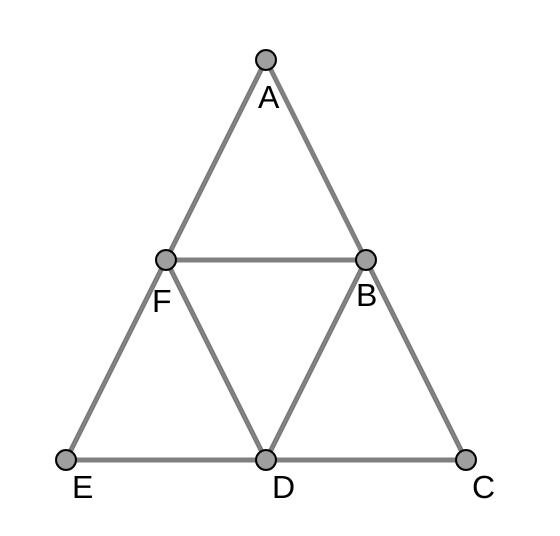
\includegraphics[width=30mm]{sungraph}
			\end{figure}
			\item Bizonyítás arra az esetre, ha a duális gráfban van Hamilton-kör (Goddard, Henning)
			\item Bizonyítás arra az esetre, ha minden csúcs foka páratlan. (Goddard, Henning)
		\end{itemize}
\end{frame}

\begin{frame}{Átfogalmazások}
	\begin{itemize}
		\item Minden egyszerű, háromszögelt, legalább $4$ csúcsú síkgráfban létezik
			olyan részgráf, amely minden kerékből tartalmaz élt. (Ekvivalens a sejtéssel.)
			\begin{figure}[h]
				\centering
				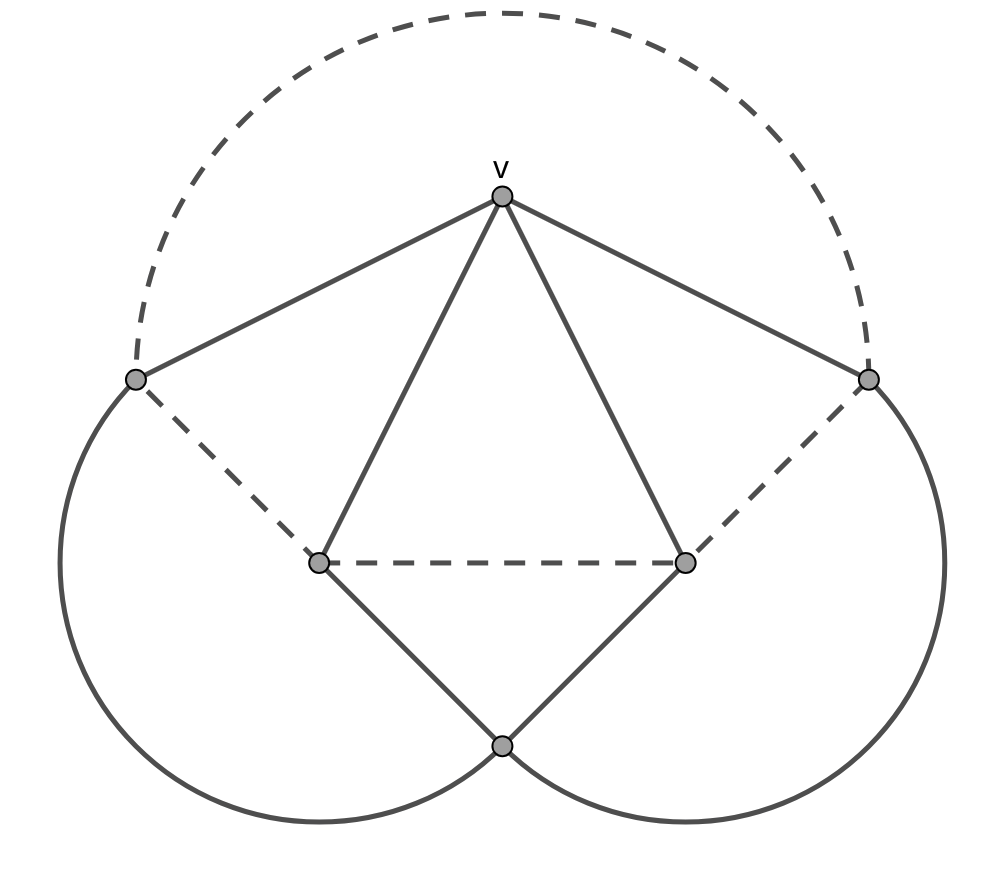
\includegraphics[width=30mm]{wheel}
			\end{figure}
		\item Minden $3$-reguláris, $2$-élösszefüggő, legalább $4$ csúcsú síkgráfban létezik
			olyan $2$-faktor, amely nem tartalmaz lapot. (Elégséges a sejtés igazolásához.)
	\end{itemize}
\end{frame}

\begin{frame}{Eredmények}
	\begin{itemize}
		\item Ha létezik a gráfban $2k+2$ hosszú kört nem tartalmazó $2$-faktor, akkor létezik
		megfelelő színezés.
		\item Ha egy négyszögelés által meghatározott két hipergráfnak létezik jó színezése,
		akkor az eredetinek is. Akkor és csak akkor létezik a hipergráfoknak jó színezése,
		ha a megfelelő segédgráfban van feszítő Euler részgráf.
		\begin{figure}[h]
			\centering
			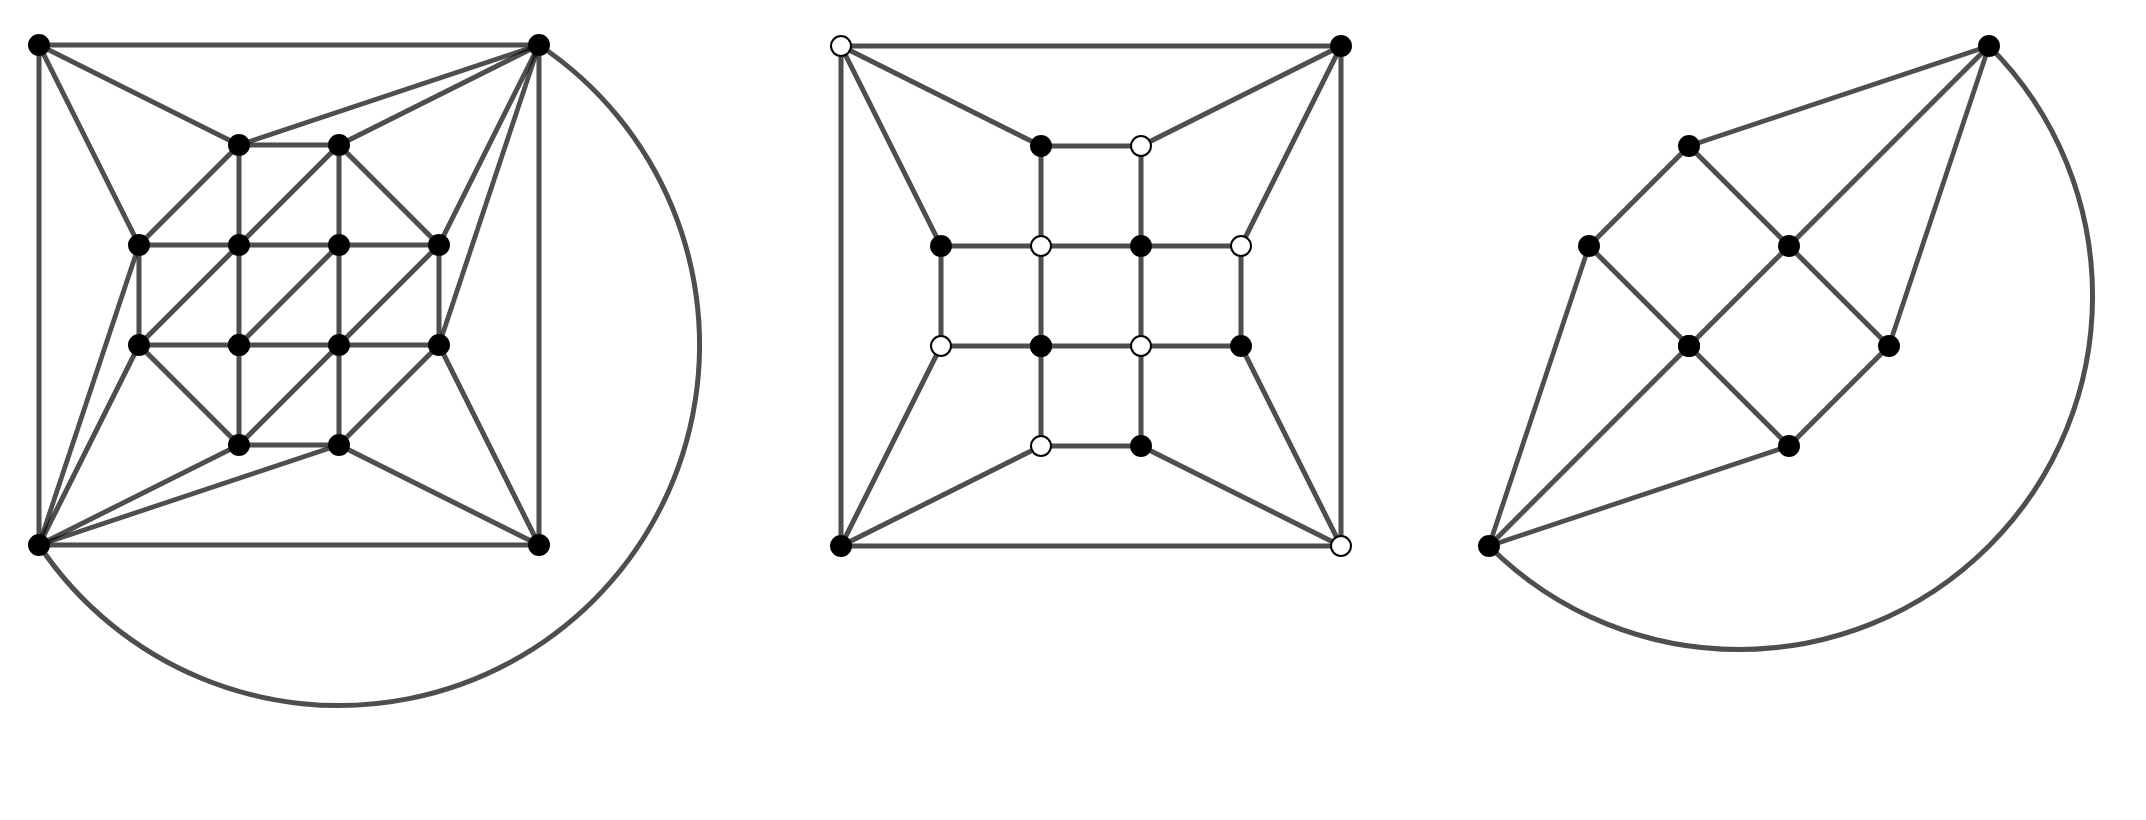
\includegraphics[width=100mm]{hypergraph2}
			\label{fig:sungraph}
		\end{figure}
	\end{itemize}
\end{frame}

{
	\usebackgroundtemplate{
\includegraphics[width=1.0\paperwidth]{theme.jpg}}
	\begin{frame}[plain]
		\begin{center}
			\textcolor{white}{\Huge{Köszönöm a figyelmet!}}
		\end{center}
	\end{frame}
}




\end{document}
